\section{Design}

%以下两图展示了nfactor系统的基本架构。nfactor框架将统一的运行时系统组成cluster。在这个nfactor cluster内,细粒度的流管理可以被快速的执行。这个cluster由一个轻量级的控制器进行控制以实现动态扩展,和开启流迁移以及容错。

Figure \ref{fig:runtime} and \ref{fig:runtime-arch} daemonstrate the basic architecture of NFActor framework. NFActor framework composes uniform runtime systems into a cluster. Within this cluster, fine-grained flow managmeent tasks could be quickly executed. This cluster is controlled by a lightweight controller for dynamic scaling and inititiating flow management tasks, including flow migration and fault tolerance.

%nfactor的设计遵循了以下几个原则。
The design of NFActor framework follows the following principles.

\begin{itemize}

%第一,低开销。在提供复杂流管理的同时,nfactor也必须高速的处理数据包。因此,nfactor为每一个流所提供的execution context必须是一个轻量级的抽象,它不能对正常的NF处理产生比较大的性能影响。The execution context of nfactor framework是利用actor programming model 进行构建的。我们实现了自己的actor programming model库,从编程的角度考虑,消息传递的开销仅相当于一次函数调用。

\item \textbf{Low Overhead.} While providing compliated flow management tasks, the runtime system of NFActor framework must be able to process packets at high speed. Therefore, the execution context that NFActor created for each flow must be a lightweight abstraction, it should not compromise the processing speed of a NF. In NFActor, this execution context is constructed using actor programming model. We implement our own actor programming model to minimize the overhead associated with the execution context.

%第二,效率。 为了适应高速nfv系统的需求,nfactor所提供的流管理必须十分高效。在高速nfv系统中,一个NF每秒钟需要处理几百万个包,并控制几万流。在如此高速的吞吐量下实现流管理功能,这就要求nfactor避免使用内核网络协议栈,以避免上下文切换的的开销。在nfactor系统中,所有的数据处理,无论是dataplane的数据包还是actor发送的远程消息,都是利用高速的包IO (DPDK)来实现的。

\item \textbf{Efficiency.} To accomodate the need of high speed NFV systems, the flow management tasks of NFActor must be highlighy efficient. In high speed NFV systems, a NF may process millions of packets every second and handle tens of thousands of flows. To achieve high efficiency, NFActor completely abandoned using kernel networking stack to avoid the overhead of context switching. In NFActor, all the data, whethere it's data plane packet or remote actor messages, are transmitted through high-speed packet I/O (i.e. DPDK).

%第三,可扩展性。现代nfv系统必须具有良好的可扩展性,以适应不断变化的网络流量的需求。为了实现良好的可扩展性,nfactor系统提供了统一的运行时系统,并使用多个运行时系统组成nfactor cluster。在nfactor cluster内,运行时系统可以对经过自己的流进行路由管理,以实现动态的负载均衡。同时,我们也简单而快速的在不同的runtime之间传递信息,以实现高效的流管理任务。

\item \textbf{Scalability.} Modern NFV system must have good scalability, to accomodate varying network traffic. To provide good scalability, NFActor framework provides uniforms runtimes and connects multiple runtimes into a NFActor cluster. Within this cluster, the runtime system could manage output route for each flow that passes through it, to achieve dynamic load balancing. The uniform runtime design also faciliatates message passing among different runtimes, to achieve efficient flow management tasks.

\end{itemize}

\subsection{Runtime Cluster}


\begin{figure}[!t]
\begin{subfigure}[t]{0.30\linewidth}
   \centering
   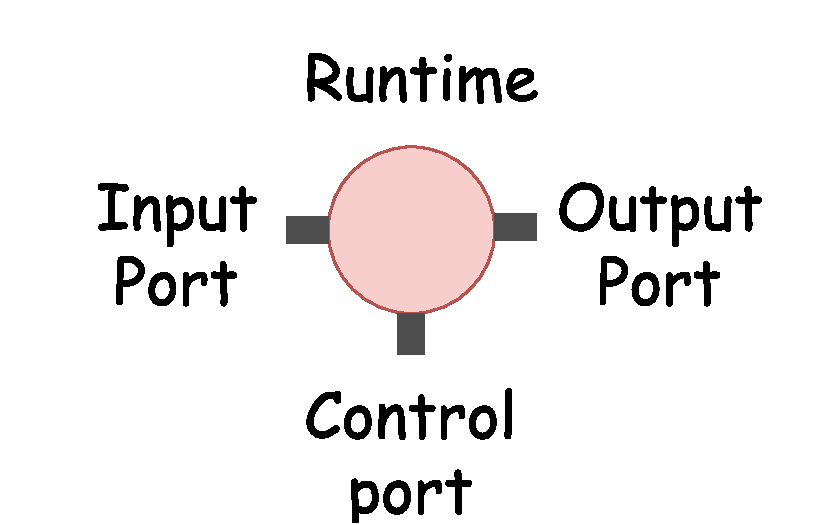
\includegraphics[width=\columnwidth]{figure/nfactor-runtime-with-port.pdf}
   \caption{A runtime with three ports.}\label{fig:runtime-with-port}
  \end{subfigure}\hfill
  \begin{subfigure}[t]{0.69\linewidth}
 \centering
   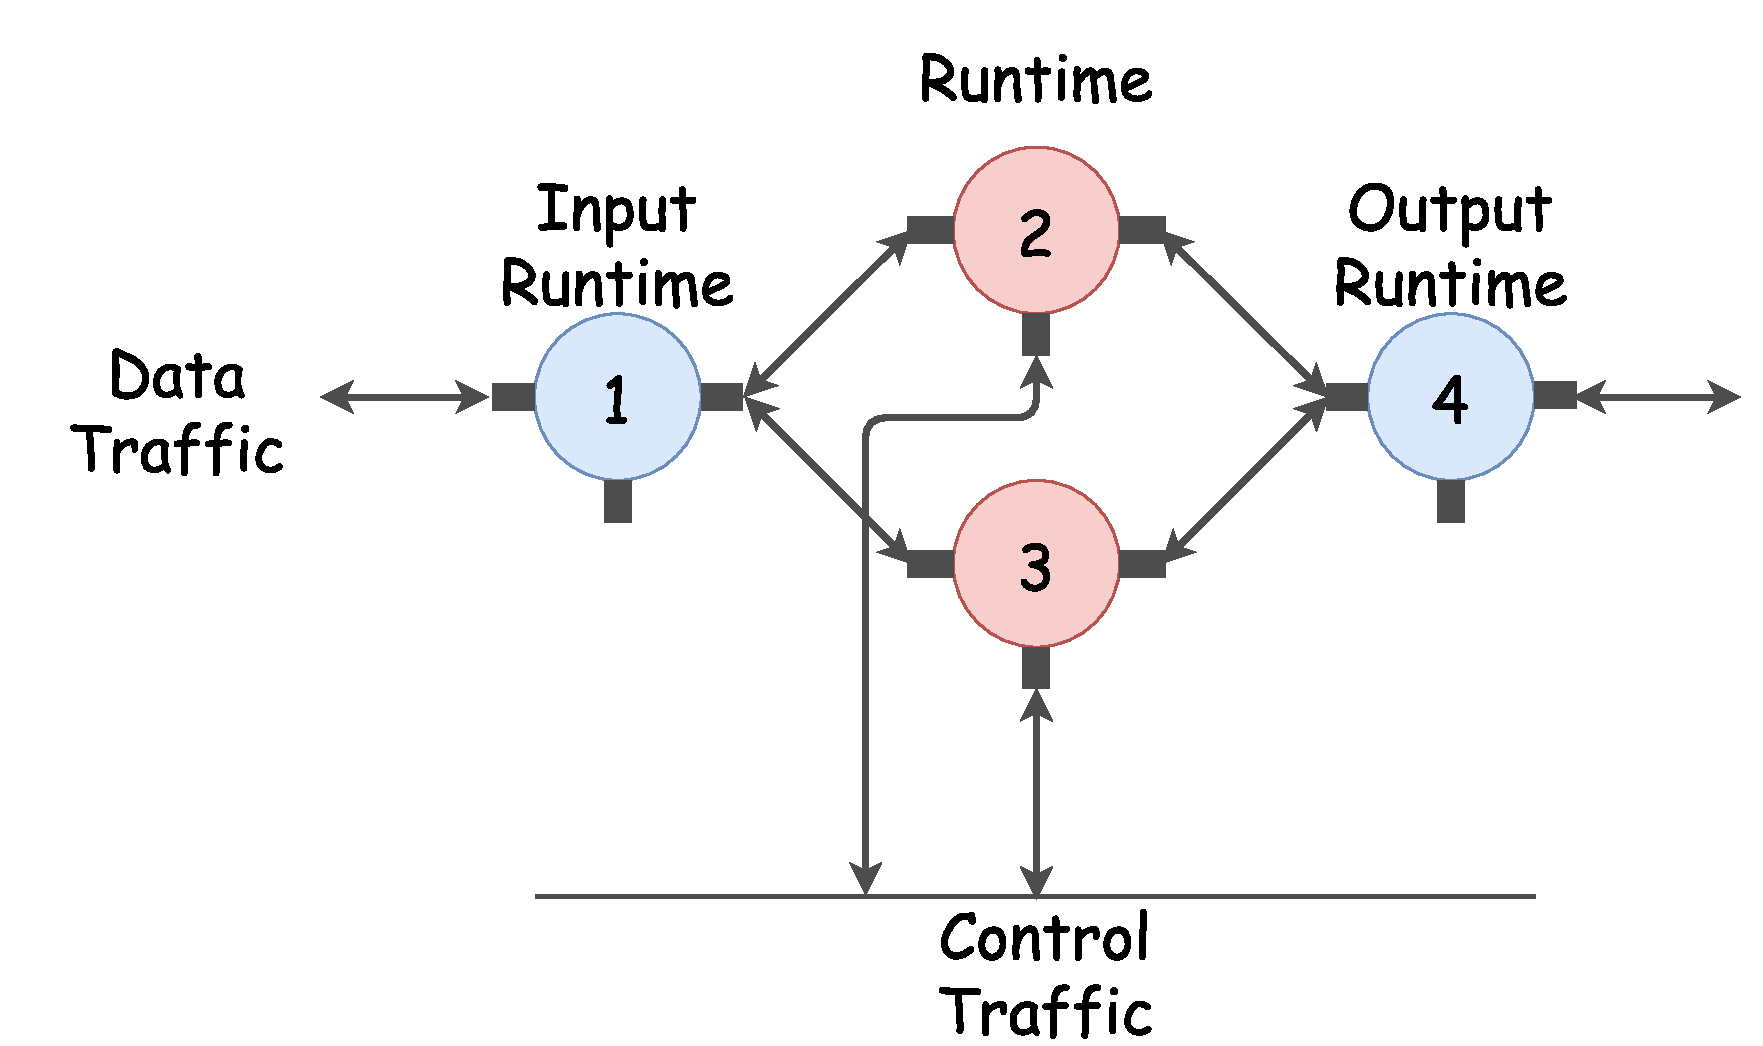
\includegraphics[width=\columnwidth]{figure/nfactor-runtime-connection.pdf}
   \caption{A minimal runtime connection.}\label{fig:runtime-with-io-runtime} \end{subfigure}\hfill
   \begin{subfigure}[t]{0.99\linewidth}
  \centering
    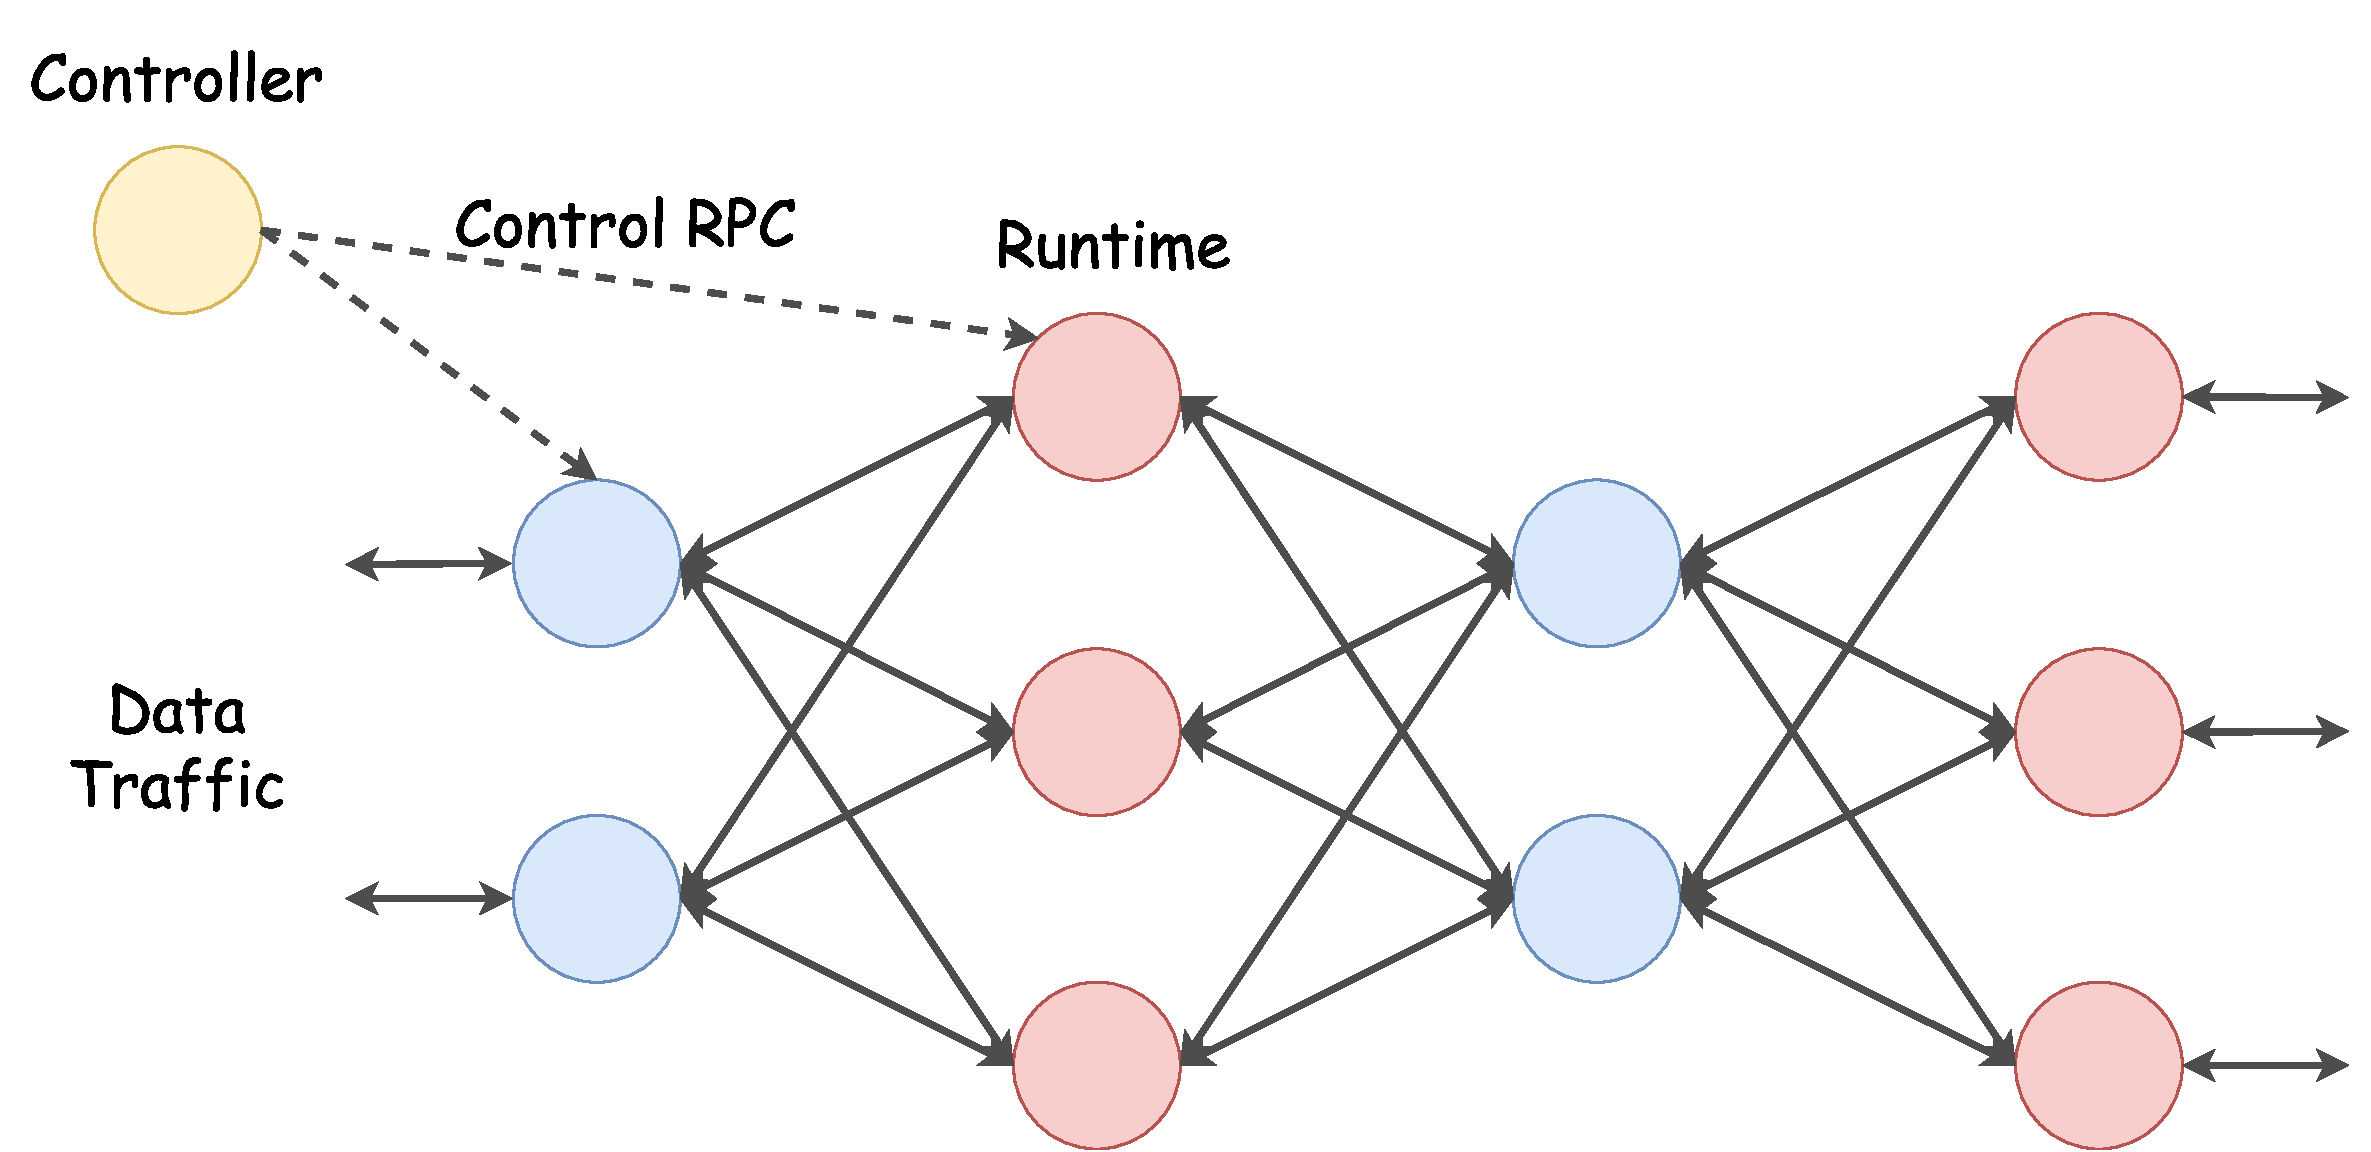
\includegraphics[width=\columnwidth]{figure/nfactor-cluster.pdf}
    \caption{A NFActor runtime cluster consists of multiple lay, controlled by a controller.}\label{fig:runtime-cluster} \end{subfigure}
 \caption{The flow migration performance of \nfactor}
\label{fig:runtime}
\end{figure}

%图1c展示了运行时cluster的基本结构。运行时cluster是由若干层运行时连接而成,并由一个轻量级的控制器利用RPC进行管理。
Figure \ref{fig:runtime-cluster} gives an example of a running NFActor cluster. The NFActor cluster consists of multiple runtimes controlled by a light-weight controller through RPC.

%图1a给出了一个runtime的基本结构。一个runtime包含三个端口。输入端口和输出端口用来接收和传递数据层的数据包。控制端口专门用来传递flow actor执行流管理任务时所生成的远程消息。输入输出端口也可以用来传递远程消息,我们在后面的章节中给出详细的解释。
Figure \ref{fig:runtime-with-port} shows the basic struture of a runtime. A runtime consists of three ports. The input and output ports are used to receive and send dataplane packets. The control port is only used to transmit remote messages when flow actor executes flow management tasks. Both input and output ports could also be used to transmit remote messages, this is further illustrated in later chapters.

%一个运行时系统自己并不能执行负载均衡以及流管理任务,它需要和其他的运行时系统进行连接才能完成这些功能。每一个运行时系统的三个端口都可以和其他多个运行是系统进行连接。图1b给出了一个能实现各种流管理功能的最小连接图。在图1b中,2号运行时系统的输入端口和输出端口分别与1号运行时系统的输出端口和4号运行时系统的输入端口相连,因此对于2号运行时系统而言,1号运行时系统时它的input runtime, 4号运行时系统时它的output runtime.同理,对于1号运行时系统而言,2号运行时系统时它的output runtime. 在NFActor framework中,运行时系统可以将自己的输出流量均匀分布在所有的输出运行时系统中。因此我们可以看到 dataplane traffic可以从图1b连接的一端进入并从另一端输出。

A runtime system could not execute any load-balacning and flow management tasks by itself. It needs to be connected with other runtimes and collaborate with those runtimes. The three ports of a single runtime system could be connected to multiple runtimes. Figure \ref{fig:runtime-with-io-runtime} gives a minimal runtime connection that is able to achieve load-balancing and flow management tasks. In figure \ref{fig:runtime-with-io-runtime}, the input and output ports of runtime 2 and 3 are connected with the output port of runtime 1 and input port of runtime 4. From the perspective of runtime 2, runtime 1 is its input runtime and runtime 4 is its output runtime. Similarly, runtime 2 is the output runtime of runtime 1. In NFActor framework, a runtime could balance its workload among all of its output runtimes. This is why the dataplane traffic could enter from one end of the connection in figure \ref{fig:runtime-with-io-runtime} and exit from the other end.

%对与2号和3号运行时系统而言,他们具有相同的input runtime和output runtime。我们将这一类运行时系统归纳入通一个layer。同一个layer的运行时系统的控制端口会被相互连接起来。同时,同一个layer的运行时系统之间可以实现快速高效的流迁移和容错。

From the perspective of runtime 2 and 3, they share the same input runtimes and output runtimes. These runtimes are classified into the same layer. The control ports of runtimes under the same layer are directly connected, so that flows could be quickly migrated and replicated among runtimes under the same layer.

%如图2所示,我们可以构建一个由multipile layers of runtime 所组成的nfactor cluster。这个cluster由一个轻量级的controller进行控制。controller可以检测每一个runtime的workload以实现动态扩展。同时,controller可以通过rpc来发起流管理任务的执行。

As shown in figure \ref{fig:runtime-cluster}, we can construct a NFActor cluster by creating multiple layers of runtimes. This runtime cluster could be controlled by a controller, which monitors the workload on each runtime for dynamic scaling. This controller could also initiate flow management tasks by sending RPC requests to selected runtimes.

\subsection{Runtime Architecture}

\begin{figure}
		\centering
		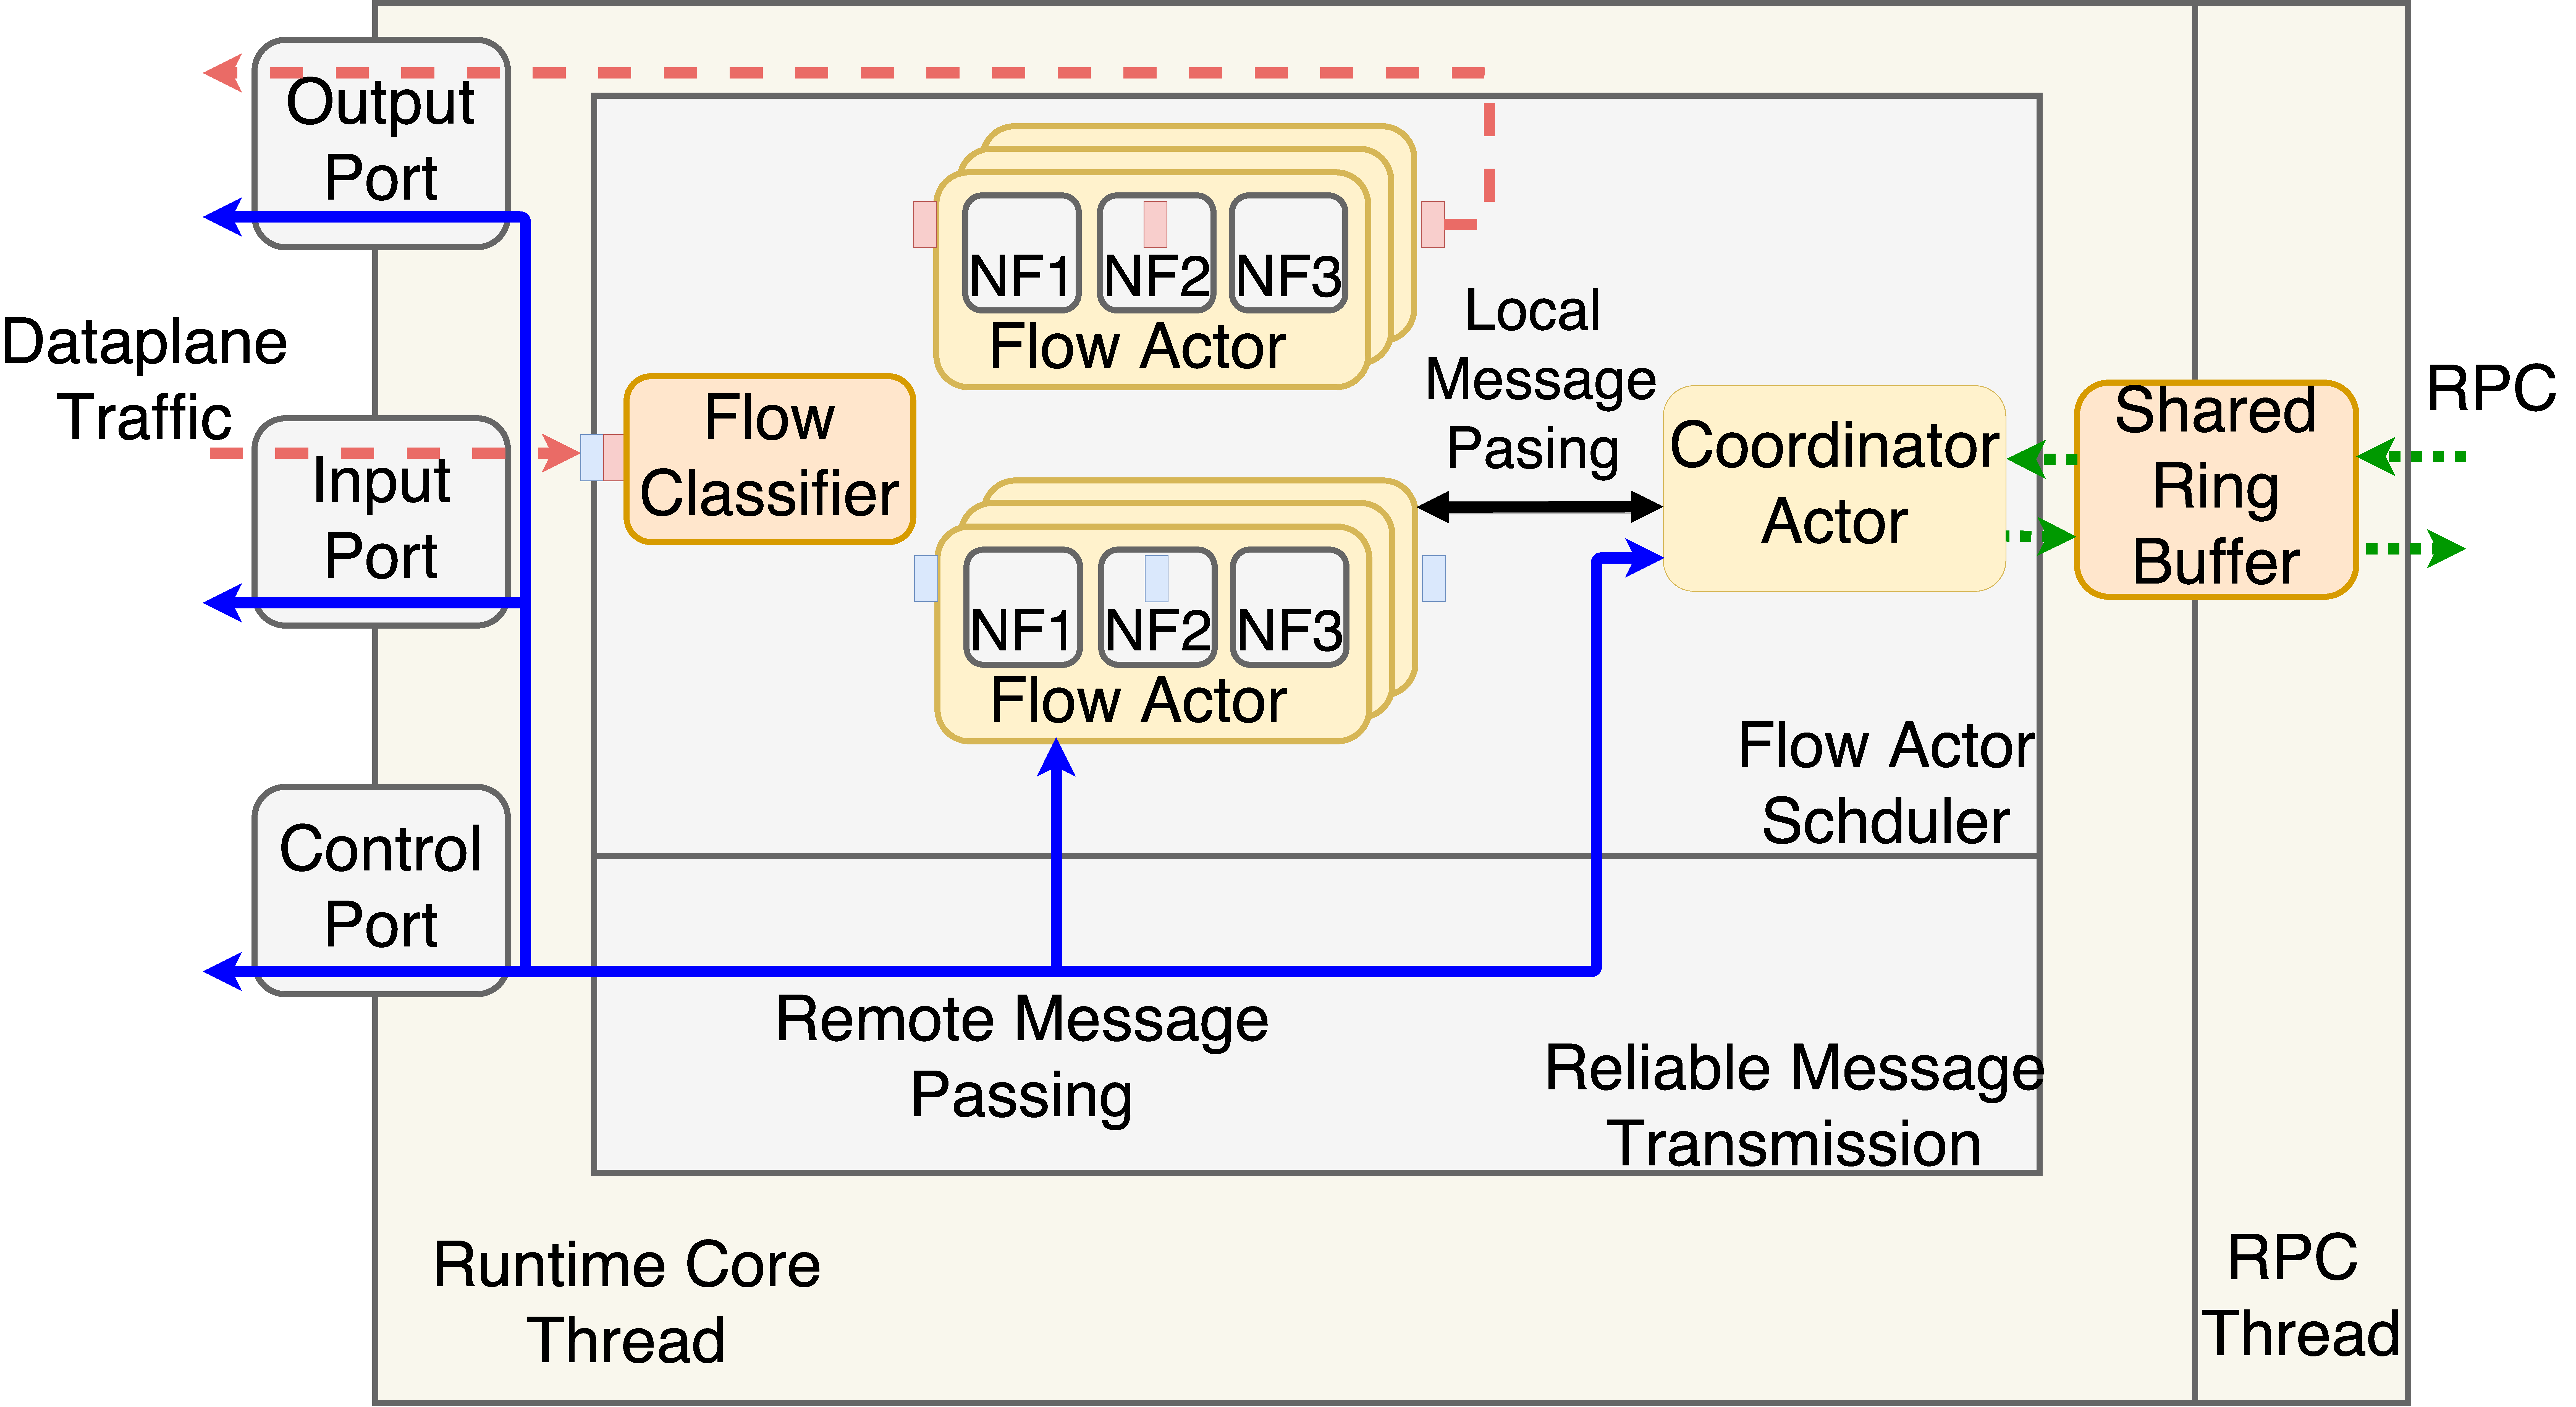
\includegraphics[width=\columnwidth]{figure/nfactor-runtime-arch.pdf}

		\caption{The internal architecture of a NFActor runtime system. }
\label{fig:runtime-arch}
\end{figure}

%图二展示了一个runtime的内部架构。一个runtime包含core thread 和rpc thread连个线程。rpc thread专门用来接收controller 发来的RPC 指令,并将这些指令利用一个共享的高速环形队列转发到core thread中。core thread里运行了两个重要的模块,分别是flow actor调度器和reliable message transmission module。这两个模块由一个模块调度器进行轮询调度。

Figure \ref{fig:runtime-arch} demonstrates the internal architecture of a runtime, which consists of an RPC thread and a core thread. The RPC thread receives RPC requests from the controller and forward these requests to the core thread using a shared ring buffer. The core thread has a flow actor scheduler module and a reliable message transmission module. Both of these two modules are scheduled to run by a round-rubin module scheduler.

%从输入端口获取的dataplane 的数据包会被直接发送给flow actor scheduler. flow actor scheduler 利用flow classifier对包进行分流。在我们当前的实现中,flow classifier使用传统的flow-5-tuple作为key来对包进行分流。flow classifier会为每一个新的流建立一个与之唯一对应的flow actor并将这个流的所有数据包交由flow actor进行处理。flow actor会将收到包依次通过一个在初始化时确定的service chain。当这个包完成处理时,flow actor会将这个数据包从输出端口送出。流调度器还会定时调度一个coordinator actor。这个coordinator actor负责从共享队列里提取rpc命令并执行rpc命令。

The core thread polls dataplane pacekts from the input port and forwards them to flow actor scheduler. The flow actor scheduler uses a flow classifier to classify packets into different flows. In our current implementation, the flow classifier uses tranditional flow-5-tuple (i.e. IP destination address, IP source address, transmission layer protocol, source port and destination port) to classify flows. Flow classifier creates an unique flow actor for each new flow, and forwards all the packets of a flow to its flow actor. The flow actor processes the packet by passing the packet through a pre-determined service chain at runtime initialization time. When the packet finishes processing, it is delivered to the output port. The flow actor scheduler also peoriodically schedules a coordinator actor, which is responsible for fetching RPC requests from the shared ring buffer and executes these requests.

% 同一个runtime上的flow actor和coordinator actor之间可以发送本地消息进行通信。不同runtime 上的actor可以利用reliable message transmission module来发送远程消息。在NFActor framework里,我们为每一个runtime分配一个唯一的runtime id,并为每一个actor分配一个唯一的actor id。 当进行远程actor message 传输时,发送actor只需要向reliable message transmission module指名接收actor 的id 以及接收actor所在的runtime id。消息就可以被可靠的传输出去。
Flow actor and coordinator actor on the same runtime could directly pass messages with each other. Actors on different runtime use reliable message transmission module to send remote messages. In NFActor framework, we assign a unique ID for each runtime and each actor. When an actor sends a remote message, it only needs to specify the actor ID of the receiver and the runtime ID of the receiver. The message is then delivered reliably to remote side by the reliable message passing module.


%一个runtime上只创建一个core thread的设计主要是为了减小使用actor programming model的overhead. 在我们最初的设计中,我们使用libcaf actor来构建flow actor。libcaf 库会建立自己的多个工作线程。flow actor会直接被这些工作线程进行调度。为了将从高速包IO端口获得包并发送给flwo actor,我们不得不再创建一个单独的轮询线程。在这种设计下,我们发现整个系统的最大吞吐量不会随着libcaf工作线程的增加而增大,因为前方的轮询线程会成为一个瓶颈。因此我们直接抛弃了多个工作线程的设计,采用一个core thread 来poll数据包,并调度flow actor。这种架构可以让我们对actor programming model采取很激进的优化,我们可以将消息传递通过函数调用进行直接实现,而不需要考虑同步问题。然后系统的scalability可以用过增加runtime的数目来实现。我们可以在evaluation章节中看到,这样的设计可以取得令人满意的效果。

The reason that a runtime has only one core thread is to improve resource utilization rate and minimize the overhead of using actor programming model. In our initial prototype implementation, we used LIBCAF \cite{caf} library to construct flow actors. LIBCAF library creates multiple worker threads and schedules flow actors to run onthese worker threads. In order to poll from the input port and send packet to flow actor, we have to create another polling thread. Under this design, we found out that the maximum throughput of a single runtime does not increase when the number of LIBCAF worker thread increases, because the polling thread has always been a bottleneck. Therefore, we abondan the multi-worker-thread design and use a single core thread to poll packets and schedule flow actors. This architecture allows us to perform aggressive optimization of actor programming model \ref{}. In the mean time, we can still maintain the scalability of the system by launching more runtimes. We show in evaluation section that this architecture could achieve satisfactory performance.

\subsection{Control RPCs}

\subsection{NF Module}

\subsection{Load Balancing}

\subsection{Flow Management}
\subsubsection{Flow Migration}
\subsubsection{Flow Replication}

\subsection{Dynamic Scaling}
